%%%%%%%%%%%%%%%%%%%%%%%%%%%%%
%Since : 2019/04/03
%Update: 2020/04/22
% -*- coding: utf-8 -*-
%%%%%%%%%%%%%%%%%%%%%%%%%%%%%

\chapter{Excelによる統計処理1}
\setcounter{num_prac}{0}

\section{目的}

Excelの操作を通し,データ処理の基礎とグラフの作成の仕方を学ぶ.

\section{統計とは}

統計や確率は様々な場面で用いられています.
それはなぜでしょうか.
一つの理由は,全体の特徴もしくは規則性を捉えるためです.
皆さんは,大学受験で大学の偏差値や合格者のセンター試験の平均点などを調べたのではないでしょうか.
偏差値やセンター試験の平均点は立派な統計によって得られた量です.
これらの数値は,大学の合格者の集団の特性を表しています.
今後,卒業研究はもちろん就職してからも大量のデータを扱い,集団の特性や規則性を調べることになると思います.
この演習を通じ,統計の基礎とExcelによる簡単な統計処理を身につけてください.
しかし,統計やそれと関わる機械学習を本気で使うのであればRやPythonといったプログラミング言語を学ぶ必要があります.

\section{データ}
\subsection{データセット}

$N$個の値からなるデータセットがあるとするとそのデータセット$X$は次のように表されます.
\begin{equation}
    \label{eq:2}
    X = \{x_1, x_2, ..., x_N\}.
\end{equation}

\subsection{データの保存形式}

データを保存するためのデータ形式は様々ありますが,この演習ではcsvファイルとxslxファイルを用います.
csvファイルは,Comma-Separated Valuesファイルの略です.
その名の通り,csvファイルの中身は,データがカンマで区切ってあるだけのテキストファイルです.
単なるテキストファイルですので,どのようなコンピュータを使っている人でも必ず見ることができます.
csvファイルはExcelなど表計算ソフトが入っていれば,表計算ソフトに関連付けされています.
ただし,csvファイルはあくまでも単なるテキストファイルですので,表計算ソフトによる関数による自動計算,作成したグラフ,文字の装飾,表の罫線などは保存されません.
xslxファイルはExcel2007以降で標準的に用いられるファイルです.データだけではなく,関数による自動計算,作成したグラフ,文字の装飾,表の罫線なども保存されます.
この演習では,データはcsvファイルで提供します.
\textbf{演習結果の保存は必ずxslxファイルにしましょう.}

\section{統計量}

\subsection{様々な統計量}

例えば,表\ref{tab:sample}に示すデータがあったとします.
このデータの特徴は何でしょうか.
といきなり言われても困りますよね.
そこで, データの特徴を表すために統計学の力を借りることが多くあります.
データの特徴を表す統計学的な方法により求められた量のことを統計量と言います.
今回用いる統計量は,平均,中央値,分散,標準偏差です\footnote{特に,これらの統計量は基本統計量と呼ばれます.}.

\begin{table}[tb]
    \caption{データ}
    \centering
    \begin{tabular}{cccccccccc}
       82 & 66 & 39 & 66 & 54 & 56 & 58 & 72 & 53 & 60 \\
       69 & 79 & 71 & 68 & 50 & 68 & 61 & 66 & 74 & 77 \\
       74 & 72 & 73 & 56 & 47 & 59 & 56 & 76 & 69 & 67 \\
       87 & 66 & 57 & 45 & 84 & 53 & 47 & 52 & 49 & 74 \\
       83 & 69 & 87 & 61 & 59 & 64 & 66 & 69 & 79 & 68 \\
       55 & 68 & 50 & 66 & 60 & 69 & 60 & 58 & 83 & 72 \\
       74 & 79 & 65 & 77 & 52 & 65 & 48 & 56 & 76 & 65 \\
       63 & 62 & 63 & 77 & 72 & 68 & 69 & 59 & 63 & 82 \\
       63 & 68 & 80 & 61 & 48 & 58 & 55 & 61 & 54 & 66 \\
       69 & 56 & 79 & 61 & 62 & 61 & 65 & 65 & 75 & 69 \\
    \end{tabular}
    \label{tab:sample}
\end{table}

\paragraph{平均}
平均$\mu$は集団の値の重心を表す最も頻繁に用いられる統計量です.
平均は次の式で表されます.
\begin{equation}
    \mu = \frac{1}{N} \sum_{i=1}^{N} x_i.
\end{equation}
皆さんおなじみの平均です.表\ref{tab:sample}のデータの平均は65.09です.


\paragraph{中央値}
中央値はデータを大きさ順で並べ替えて,順番としてちょうど真ん中にあたる値のことです.
例えば,$\{1, 4, 5, 7, 8\}$のようなデータがあったとすると,中央値は順番的に真ん中の5となります.
例のデータの数は奇数でしたので,順番としての中央を決定できましたが,データの数が偶数の場合はどうしたら良いでしょうか.
例えば,$\{1,3,4,5,7,9\}$のようなデータがあったとすると,ちょうど真ん中の値はありません.このような場合は,真ん中の2つの値,4と5を足して2で割った値,すなわち4.5が中央値となります.
表\ref{tab:sample}のデータの中央値は65.5です.
表\ref{tab:sample}のデータの場合は,平均と中央値にあまり差がないので,中央値がある必要性が分からないかもしれませんが,中央値は,平均に対して利点があります.
後のほど行う演習で確かめましょう.

\paragraph{分散と標準偏差}
分散はデータのばらつき具合を表します.
分散は次の式で表されます.
\begin{equation}
    \sigma^2 = \frac{1}{N} \sum_{i=1}^{N} (x_i - \mu)^2.
\end{equation}
分散の平方根を標準偏差といいます.
表\ref{tab:sample}のデータの分散は約102で標準偏差は約10.1です.


\subsection{Excelによる統計量の計算}

統計量の一つである総和をExcelで計算してみます.
手順は次のとおりです.

\begin{enumerate}
    \item データを入力します.今回は,図\ref{fig:sum}のようにA列に1, 2, 3, 4, 5と入力してください.
    \item 総和を入力したいセルを選択する.
    \item ``=SUM(''と入力する.
    \item 総和を計算したいセルをマウスで選択する.
    そうすると``(''の後ろにセル番号が入力されます(図\ref{fig:sum}).
    また,データのセル番号を直接入力することで,マウスで選択する操作と同様のことができます.
    例の場合では,セルA1からA5までの総和なので``=SUM(A1:A5)''と書きます
    \footnote{データを選択する方法はいくつかあります.
      皆さんの慣れた方法でやってください.}
    \footnote{Excelも自動でいろいろやってくれるので,閉じカッコが保管される場合もあります.
      臨機応変に対応してください.}.
    \item ``)''を入力する.
\end{enumerate}

同じやり方で,平均,分散,標準偏差が計算できます.
平均なら``SUM''の部分を``AVERAGE''に変えます.統計量とExcelの関数の関係を表\ref{tab:funcs}に示します
\footnote{分散と標準偏差に関連する関数は複数あります.
  それぞれ意味が違います.
  それぞれの意味はこの講義で扱う範疇を超えているので説明しません.
  興味がある人は調べてみましょう.}.

\begin{figure}[htbp]
    \begin{minipage}{0.5\hsize}
        \centering
        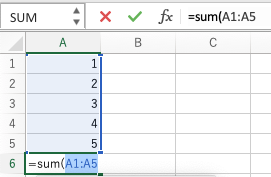
\includegraphics[width=6cm]{chap1/sum.png}
        \caption{総和を計算したいセルを選択した状態.}
        \label{fig:sum}
    \end{minipage}
    \begin{minipage}{0.5\hsize}
        \centering
        \makeatletter
        \def\@captype{table}
        \makeatother
        \caption{代表値とExcelの関数}
        \begin{tabular}{|c|c|}
          \hline
          総和     & SUM\\ \hline
          平均     & AVERAGE\\ \hline
          中央値   & MEDIAN \\ \hline
          分散     & VAR.P\\ \hline
          標準偏差 & STDEV.P \\ \hline
          最大値   & MAX \\ \hline
          最小値   & MIN \\ \hline
        \end{tabular}
        \label{tab:funcs}
    \end{minipage}
\end{figure}

\section{度数分布表とヒストグラム}

\subsection{度数分布表,ヒストグラムとは}

生データを並べただけでは,それが持つ特徴を直感的に理解することは難しいです.
そこで,データの整理の方法の一つに,度数分布表があります.
度数分布表は,データの取りうる範囲をいくつかの階級に分け,それぞれの階級にあるデータの数 (度数) を表したものです.
表\ref{tab:hist}に度数分布表の例を示します.

この度数分布表を図で表したものがヒストグラム(図\ref{fig:histogram})です.
ヒストグラムの横軸は階級を表し,縦軸が度数を表します.
つまり,棒の長さ(面積)が階級に占めるデータの多さを表すことになります.
ヒストグラムの形状を分布といいます.
分布の形状はデータの特徴として非常に重要です.

\begin{figure}[tb]
    \begin{minipage}{0.5\hsize}
        \makeatletter
        \def\@captype{table}
        \makeatother
        \centering
        \caption{度数分布表}
        \begin{tabular}{c|c}
          階級       & 度数 \\ \hline
          0から10    & 0 \\
          11から20   & 0 \\
          21から30   & 0 \\
          31から40   & 1 \\
          41から50   & 8 \\
          51から60   & 23\\
          61から70   & 40\\
          71から80   & 21\\
          81から90   & 7 \\
          91から100  & 0 \\
          100以上    & 0 \\
          合計       & 100
        \end{tabular}
        \label{tab:hist}
    \end{minipage}
    \begin{minipage}{0.5\hsize}
        \centering
        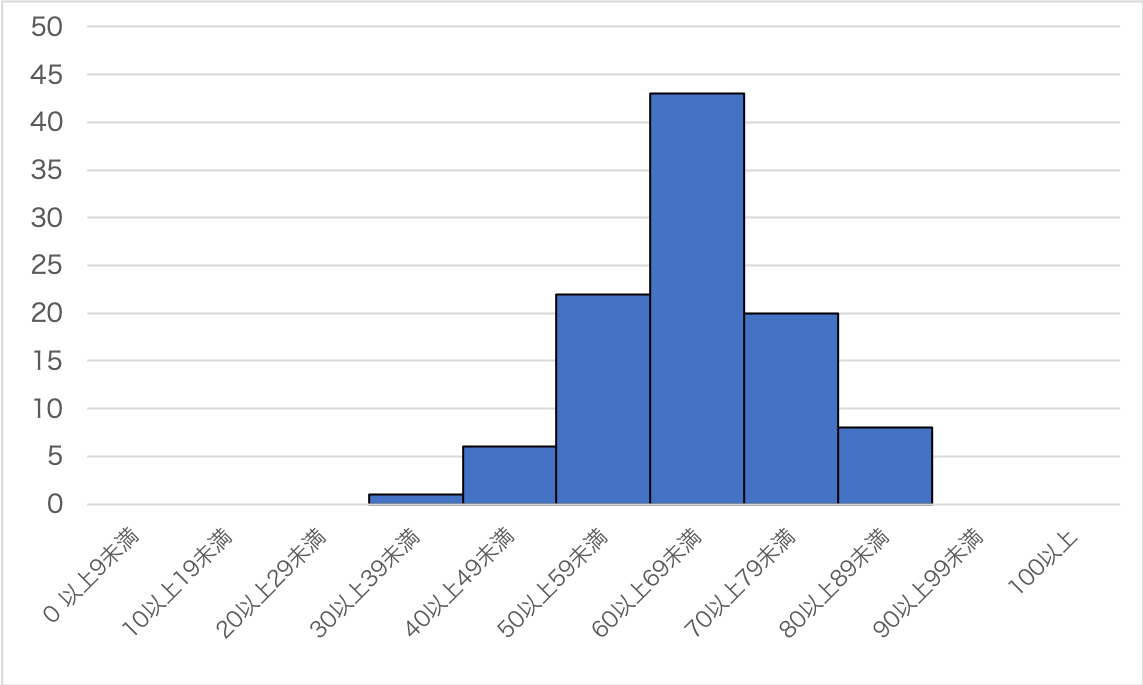
\includegraphics[width=6cm]{chap1/hist.png}
        \caption{ヒストグラム}
        \label{fig:histogram}
    \end{minipage}
\end{figure}

\subsection{度数分布表の作成}
\label{sec:make_freq}

Excelを用い,データ (表\ref{tab:sample})から図\ref{fig:freq}のような度数分布表を作るためには次の手順が必要です.

\begin{enumerate}
    \item まず,図\ref{fig:before_freq}のA列のようにExcelにデータを入力します.
    表\ref{tab:sample}のデータはfreq.csvに入っていますので,それを開くとA列にデータが表示されます.
    \item 次に階級を設定します.
    今回は,0から10,11から20,21から30,31から40,41から50,51から60,61から70,71から80,81から90,91から100という階級にします.
    \item 度数分布表を図\ref{fig:before_freq}に作成します.
    ここではまだ度数は空欄になっています.
    Excelの度数分布作成の機能の都合上,図\ref{fig:before_freq}のように階級の上限を階級の区切りとして入力しておきます.
    \item 図\ref{fig:select_cells_freq}のように度数を入力したいセルを選択します.
    \item 数式を入力するフォーム (数式バー) に``=FREQUENCY(''と入力します.
    \footnote{``COUNTIFS''という関数を使っても度数分布表を作ることが可能です.}
    \item データを選択します.そうすると,図\ref{fig:select_data_freq}のようにデータがあるセル番号が入力されます.
    \item ``,''を入力したあと,各階級の上限が入力されたセル(今回は階級の区切の列)を選択します.そうすると,図\ref{fig:select_classes_freq}のようにセル番号が入力されます.
    \item ``)''を入力します.
    \item ここが重要です.Ctrl + Shift + Enterを押します.
    \item 合計は先程用いた``sum''を用いて計算します.そうすると,図\ref{fig:freq}のような度数分布表が出来上がります.
\end{enumerate}


\begin{figure}[htbp]
    \begin{minipage}{0.5\hsize}
        \centering
        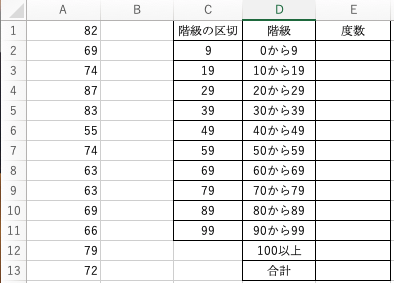
\includegraphics[width=6cm]{chap1/before_freq.png}
        \caption{Excelで作成した度数分布表}
        \label{fig:before_freq}
    \end{minipage}
    \begin{minipage}{0.5\hsize}
        \centering
        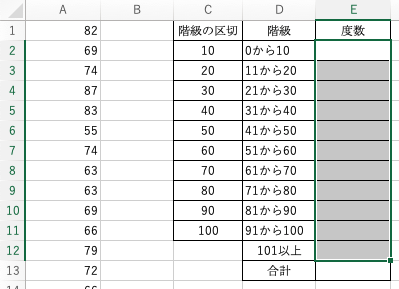
\includegraphics[width=4cm]{chap1/select_cells_freq.png}
        \caption{度数を入力するセルを選択した状態}
        \label{fig:select_cells_freq}
    \end{minipage}
\end{figure}


\begin{figure}[htbp]
    \begin{minipage}{0.5\hsize}
        \centering
        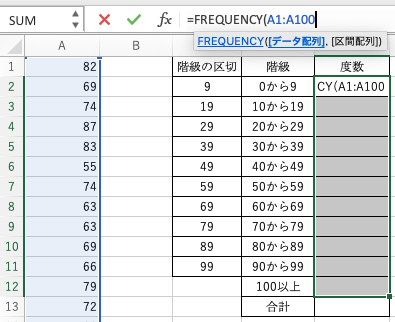
\includegraphics[width=6cm]{chap1/select_data_freq.png}
        \caption{データを選択した状態}
        \label{fig:select_data_freq}
    \end{minipage}
    \begin{minipage}{0.5\hsize}
        \centering
        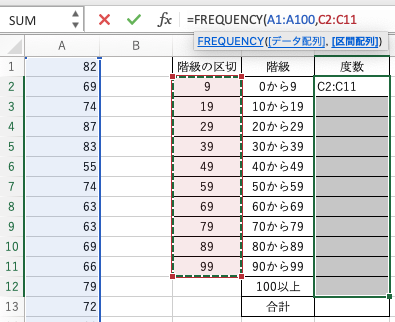
\includegraphics[width=6cm]{chap1/select_classes_freq.png}
        \caption{階級の区切りを選択した状態}
        \label{fig:select_classes_freq}
    \end{minipage}
\end{figure}

\begin{figure}[htbp]
    \centering
    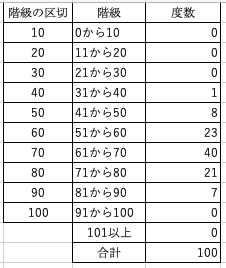
\includegraphics[width=3cm]{chap1/freq.png}
    \caption{完成した度数分布表}
    \label{fig:freq}
\end{figure}

\subsection{ヒストグラムの作成}

\ref{sec:make_freq}節で作成した度数分布表から図\ref{fig:histogram}に示すヒストグラムを作ります.
横軸は内容,縦軸は度数とします.
作る手順は次のとおりです.\footnote{ヒストグラムもかき方が多々あるので各自の好みで.}

\begin{enumerate}
    \item リボンの挿入を選びます.そうすると,グラフや図などの挿入ボタンがたくさん出てきます.
    \item 図\ref{fig:select_cells_hist}のようにグラフにしたい数値の入ったセルを選択します.
    \item リボンにある棒グラフアイコンを押し,図\ref{fig:select_barchart_hist}に示す棒グラフボタンを押します.
    そうするとヒストグラムが出来上がります.
    \item ヒストグラムの棒の幅を変えたい場合は,ヒストグラムの棒を図\ref{fig:select_bar_hist}のように選択し,図\ref{fig:select_width_hist}のGap Width (要素の間隔)を0にします.
    そうすると図\ref{fig:histogram}のようなヒストグラムが完成します.
\end{enumerate}

\begin{figure}[htbp]
    \begin{minipage}{0.5\hsize}
        \centering
  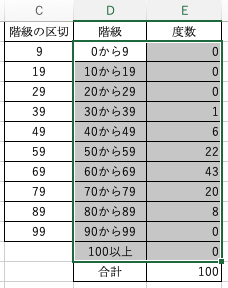
\includegraphics[width=4cm]{chap1/select_cells_hist.png}
  \caption{セルを選択した状態}
  \label{fig:select_cells_hist}
 \end{minipage}
 \begin{minipage}{0.5\hsize}
        \centering
  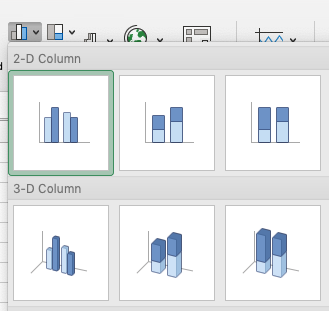
\includegraphics[width=6cm]{chap1/select_barchart_hist.png}
  \caption{棒グラフを選択する}
  \label{fig:select_barchart_hist}
 \end{minipage}
\end{figure}

\begin{figure}[htbp]
    \begin{minipage}{0.5\hsize}
        \centering
        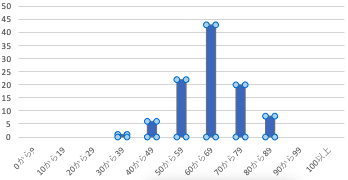
\includegraphics[width=7cm]{chap1/select_bar_hist.png}
        \caption{棒を選択した状態}
        \label{fig:select_bar_hist}
    \end{minipage}
    \begin{minipage}{0.5\hsize}
        \centering
        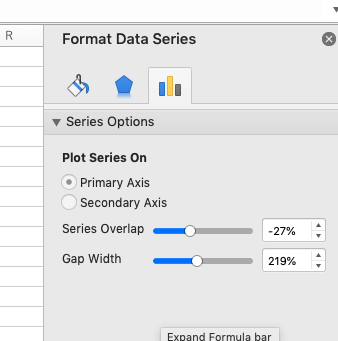
\includegraphics[width=4cm]{chap1/select_width_hist.png}
        \caption{棒の太さを選ぶ画面}
        \label{fig:select_width_hist}
    \end{minipage}
\end{figure}


\subsection{COUNTIF,COUNTIFSを用いた集計処理}

データの中から,ある条件に当てはまるものの数を数えたい場合があると思います.
例えば,表\ref{tab:countif}のような名簿から男女の数を求める場合です.
このような場合は,``COUNTIF''という関数を使います.
それではまず,表\ref{tab:countif}から,石川県出身者の人数を計算してみましょう.
\begin{enumerate}
    \item まず表\ref{tab:contif}に示すデータを図\ref{fig:countif}のように入力します.今回は,A列を番号,B列に出身県を入力します.
    \item 図\ref{fig:countif}のように人数を入れる表を作ります.
    \item まず石川県出身の人を数えたいので,人数を入れるセルに``COUNTIF(''と入力します.
    \item 出身が書かれたセルをマウスで選択します.
    そうすると``(''の後ろにセル番号が入力されます(図\ref{fig:select_cells_countif}).
    また,データのセル番号を直接入力することで,マウスで選択する操作と同様のことができます.
    この場合では,セルB2からB6までなので``=COUNTIF(B2:B6''と書きます.
    \item カンマ``,''を入力します.
    \item 図\ref{fig:operator_countif}のように条件を入力します.今回は石川県出身者の人数を数えるので,出身県のセルの内容が``石川と等しい''という条件になります.石川と等しいという条件はExcelでは,`` ``=石川`` ''と書かれます.``=''は演算子と呼ばれ,条件を表す記号です.演算子を変えることで,等しい以外に異なるなどの条件をつけることが可能です.使用できる演算子は表\ref{tab:countif_operator}に示します.
    \item 条件を入力し終えると人数が表示されます.
\end{enumerate}
うまくできたら,富山県出身者と福井県出身者の人数も計算してみましょう.

\begin{table}
\begin{minipage}{0.5\hsize}
    \centering
    \makeatletter
    \def\@captype{table}
    \makeatother
    \caption{データ}
    \begin{tabular}{|c|c|c|}
      番号& 出身県\\ \hline
      1   & 石川  \\ \hline
      2   & 福井  \\ \hline
      3   & 富山  \\ \hline
      4   & 石川  \\ \hline
      5   & 岐阜  \\ \hline
      6   & 福井  \\ \hline
      7   & 石川  \\ \hline
      8   & 大阪  \\ \hline
      9   & 石川  \\ \hline
      10  & 富山  \\ \hline
    \end{tabular}
    \label{tab:countif}
\end{minipage}
\begin{minipage}{0.5\hsize}
    \centering
    \makeatletter
    \def\@captype{table}
    \makeatother
    \caption{データ}
    \begin{tabular}{|c|c|}
      演算子 & 条件\\ \hline
      =      & 同じ\\ \hline
      <>     & 異なる\\ \hline
      >      & より大きい\\ \hline
      <      & より小さい\\ \hline
      >=     & 以上\\ \hline
      <=     & 以下\\ \hline
    \end{tabular}
    \label{tab:countif_operator}
\end{minipage}
\end{table}


\begin{figure}[htbp]
    \begin{minipage}{0.5\hsize}
        \centering
        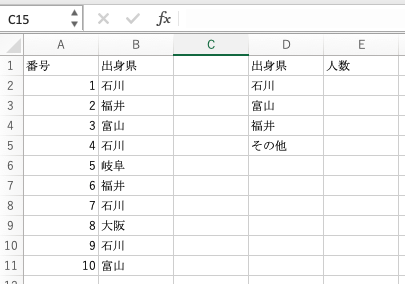
\includegraphics[width=5cm]{chap1/countif.png}
        \caption{エクセルで作成した表}
        \label{fig:countif}
    \end{minipage}
    \begin{minipage}{0.5\hsize}
        \centering
        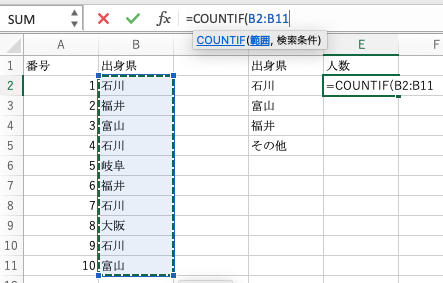
\includegraphics[width=5cm]{chap1/select_cells_countif.png}
        \caption{COUNTIFを入力しセルを選んだ状態}
        \label{fig:select_cells_countif}
    \end{minipage}
\end{figure}

\begin{figure}[htbp]
    \begin{minipage}{0.5\hsize}
        \centering
        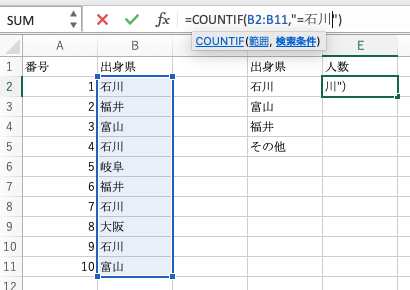
\includegraphics[width=5cm]{chap1/operator_countif.png}
        \caption{条件を入力した状態}
        \label{fig:countif}
    \end{minipage}
    \begin{minipage}{0.5\hsize}
        \centering
        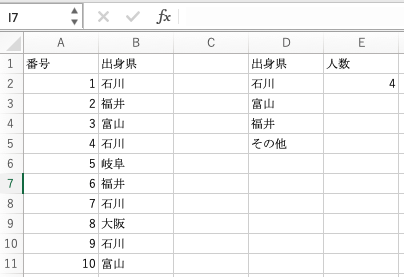
\includegraphics[width=5cm]{chap1/result_countif.png}
        \caption{出力結果}
        \label{fig:select_cells_countif}
    \end{minipage}
\end{figure}

先の方法で,石川県出身者の人数を計算できました.では,石川県,富山県,福井県以外をその他として人数を計算した場合はどうすれば良いでしょうか?この場合,3県以外なので,それぞれの県に対して異なるという条件が必要になります.つまり,条件が3つ必要です.しかし,``COUNTIF''関数は数える条件を1つしか設定できませんでした.そこで,``COUNTIFS''を用います.``COUNTIF''と``COUNTIFS''の違いは,条件が一つか,複数かの違いです.

\begin{enumerate}
    \item その他の県出身者の人数を入れるセルに``COUNTIFS(''と入力します.
    \item 出身が書かれたセルをマウスで選択します.
    そうすると``(''の後ろにセル番号が入力されます.
    また,データのセル番号を直接入力することで,マウスで選択する操作と同様のことができます.
    この場合では,セルB2からB6までなので``=COUNTIFS(B2:B6''と書きます.
    \item ``,''を入力します.
    \item 石川以外という条件``"<>石川"''を入力し,``,''を入力します.
    \item 富山以外という条件``"<>富山"''を入力し,``,''を入力します.
    \item 福井以外という条件``"<>福井"''を入力し,``)''を入力します.
    \item そうすると,入力した3条件をすべて満たすセルの数,すなわち,3県出身者以外の人数が計算されます.
\end{enumerate}

\section{演習}

\practice
アヤメデータiris.csv内にある,がく片の長さ,がく片の幅,花びらの長さ,花びらの幅についてそれぞれ平均,中央値,分散,標準偏差を求めなさい.

\practice
gaussian.csvに書かれている数値の平均と中央値を求めなさい.
そして,平均値と中央値の差について考察しなさい.
ただし,gaussian.csvは,表\ref{tab:sample}の最後のデータを500に置き換えたものです.
(ヒント:中央値の利点を調べましょう.)

\practice
glucoselevel.csvデータから度数分布表を書きなさい.ただし,階級は,60以下,60より大きく80以下,80より大きく100以下,100より大きく120以下,120より大きく140以下,140より大きく160以下,160より大きく180以下,180より大きい としなさい\footnote{http://www.qmss.jp/databank/medcomed/default.htmの血糖値データを用いました.}.

\practice
 演習3で作成した度数分布表に基づきヒストグラムをかきなさい.

\practice
第節でその他の県出身者の人数をCOUNTIFSで計算しました.実は,COUNTIFでも可能です.COUNTIFと四則演算だけでその他の県出身者の人数を計算できる数式を答えなさい.

ヒント: $10-$COUNTIF(B2:B6, "=石川")は10人中石川県出身者以外の人数になります.

\section{レポート提出}

レポートはreport1.docxの空欄を埋める形で作成し,kazuhisa.fujita@komatsu-u.ac.jpへ電子データで提出してください.データ形式はdocxもしくはpdfとします.レポートの提出期限は次回の講義日までとします.

\section{おまけ}

Excelのユーザーインターフェースを構成する各部分の名称は図\ref{fig:ui}のようになります.

\begin{figure}[htbp]
    \centering
    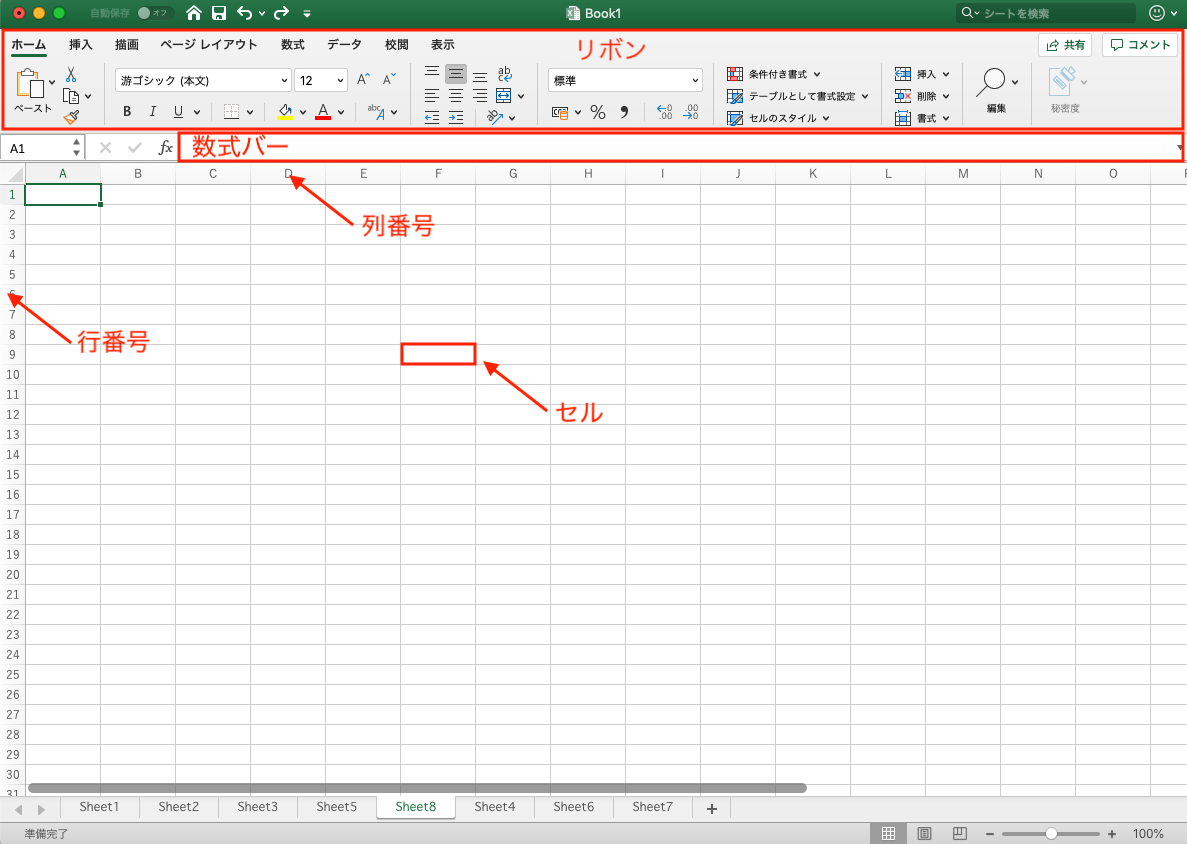
\includegraphics[width=10cm]{chap1/ui.png}
    \caption{ユーザーインターフェース}
    \label{fig:ui}
\end{figure}
